%\ifx\isEmbedded\undefined
%	% Loading common settings
%	\input{macros/common}
%	% Loading common variable definitions 
%	\input{macros/macros}
%	\begin{document} 
%\else
%\fi
%



%\setcounter{chapter}{1}

\chapter{A Simple Vision System---Revisited}
\label{chap:simple_system_revisited}
\section{Introduction}
The goal of this last chapter is to embrace the optimism of the 2020s, when we think that large-scale pretrained models can do it all, and use a pretrained end-to-end vision system in order to solve the simple visual world that we introduced in \chap{\ref{chapter:simplesystem}}.

In 2020, a number of big pretrained models (DALL-E \cite{dalle1}, GPT, chatGPT \cite{openai2023gpt4}, AutoPilot) that were solving a wide set of tasks (natural language processing, image generation, object classification, depth perception, programming, etc.) emerged. These models are trained with datasets that cover a wide set of diverse of domains that improve their generalizations and require massive amounts of computation. They can be used as is, with little to no fine tuning, or as components of more complex systems. Researchers have shown many creative ways of connecting these building blocs to produce astonishing results. However, a close analysis shows that there is still an important gap to bridge in order to build reliable and robust systems. Is the field of computer vision in the 2020s naively optimistic like in the 1960s? It does not seem to be the case, but only time will tell.

In this chapter we will revisit the simple-world problem we analyzed in \chap{\ref{chapter:simplesystem}} with a hand-crafted approach by looking for an appropriate high-performing pretrained model and applying it out-of-the-box to solve our task.

\section{A Simple Neural Network}

When we introduced the simple world in \chap{\ref{chapter:simplesystem}}, our goal was to recover the three-dimensional (3D) structure of the scene from a single image (\fig{\ref{fig:simplesystem_revisited_img1}}).

\begin{figure}
    \centerline{
        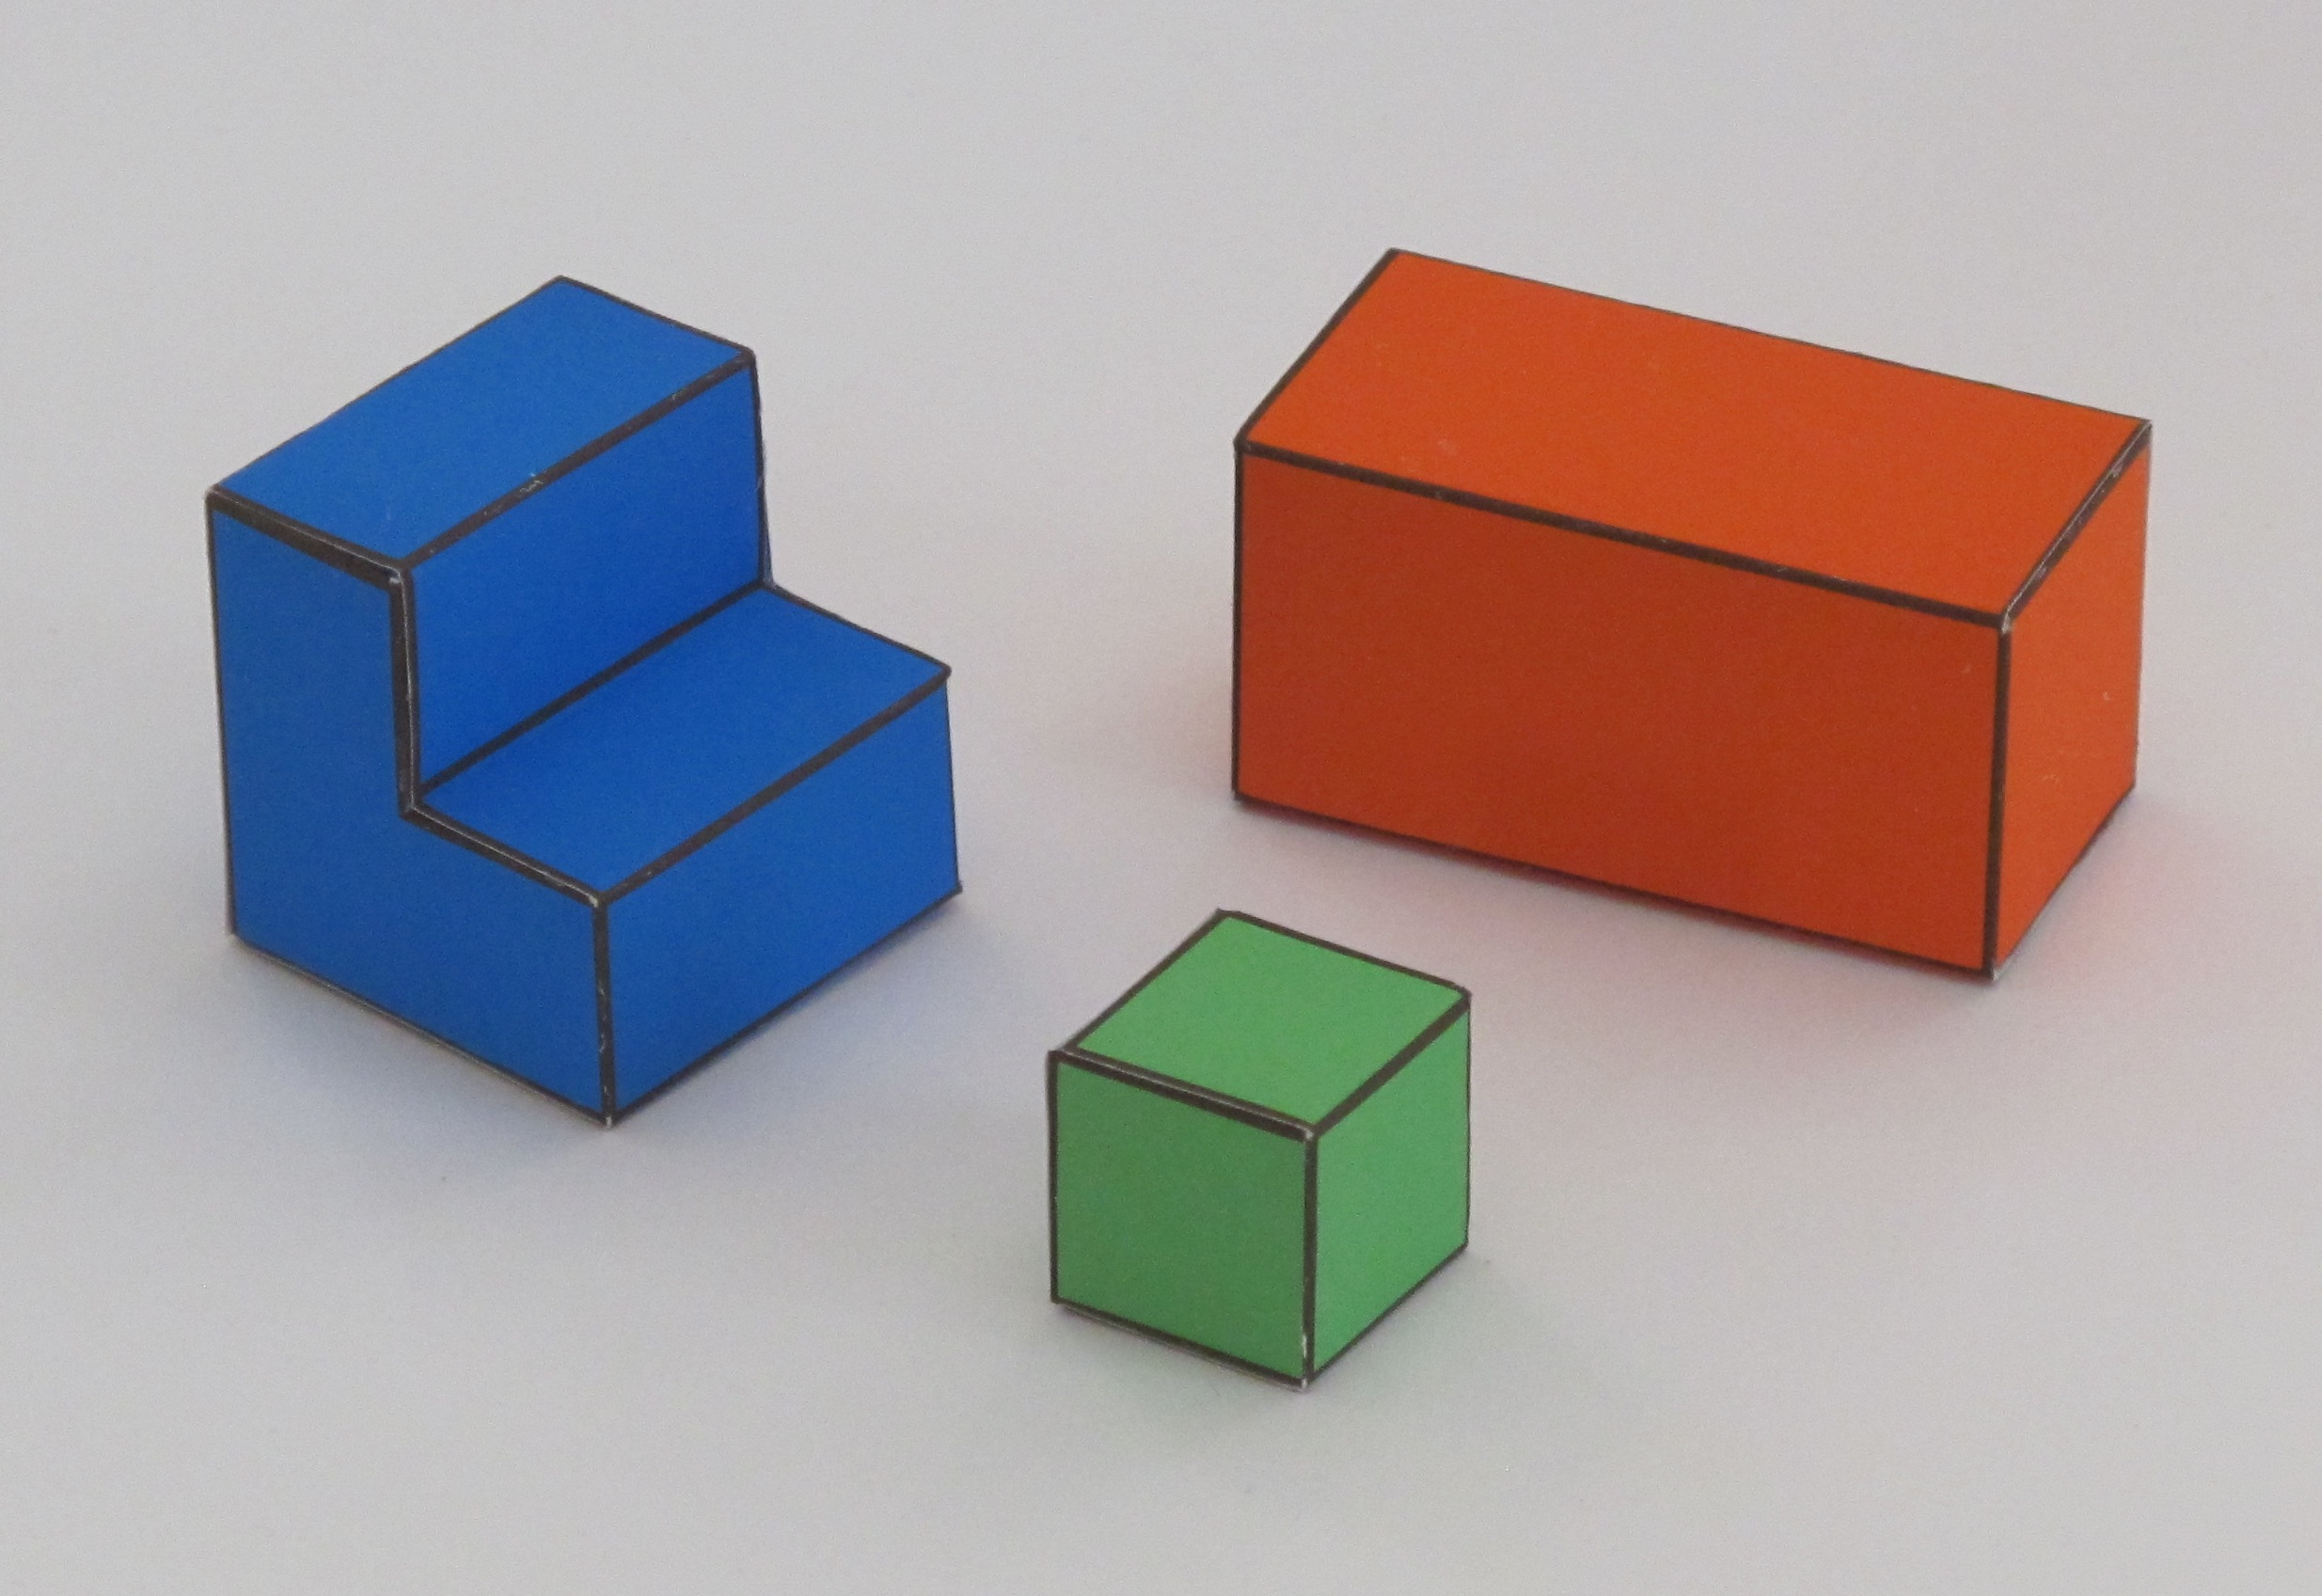
\includegraphics[width=0.4\linewidth]{figures/simplesystem_revisited/img1.jpg}
    }
    \caption{Image from the simple world.}
    \label{fig:simplesystem_revisited_img1}
\end{figure}

We derived an algorithm to recover the 3D scene structure from the first principles: we started studying the image formation process, we then reasoned where the information might be preserved, how to build a representation that makes the information explicit, and finally how to integrate all the evidence left in the image in order to recover the 3D information that was lost during the image formation process.

In this chapter, we will instead download a pretrained model that has been trained to solve the 3D perception problem from single images. The current state of the art is MiDaS \cite{Ranftl2021,Ranftl2022}. The system is a neural network trained end-to-end using a diverse set of real images that had ground truth depth information and also using stereo images.

Maybe the neural net is not so simple, but at the end, from a user's perspective, it is just a function call. Before running the system out of the box, it is worth understanding how it was trained, what the output means,  and how it can be adapted to our task.

\subsection{How Was It Trained?}
% Towards Robust Monocular Depth Estimation: Mixing Datasets for Zero-shot Cross-dataset Transfer, René Ranftl, et al. (https://arxiv.org/abs/1907.01341) 

This model has been trained using a mix of four datasets with real images. The images below (\fig{\ref{fig:examples_training_midas}}) show one sample from each dataset alongside their ground-truth depth.
% Datasets:
% ReDWeb:    https://sites.google.com/site/redwebcvpr18/
% Megadepth: https://www.cs.cornell.edu/projects/megadepth/
% WSVD:      https://sites.google.com/view/wsvd/home
% DIML Indoor: https://dimlrgbd.github.io/
% and 3D movies. While the data does not provide metric depth, we can use stereo matching to obtain relative depth

\begin{figure}
    \centerline{
        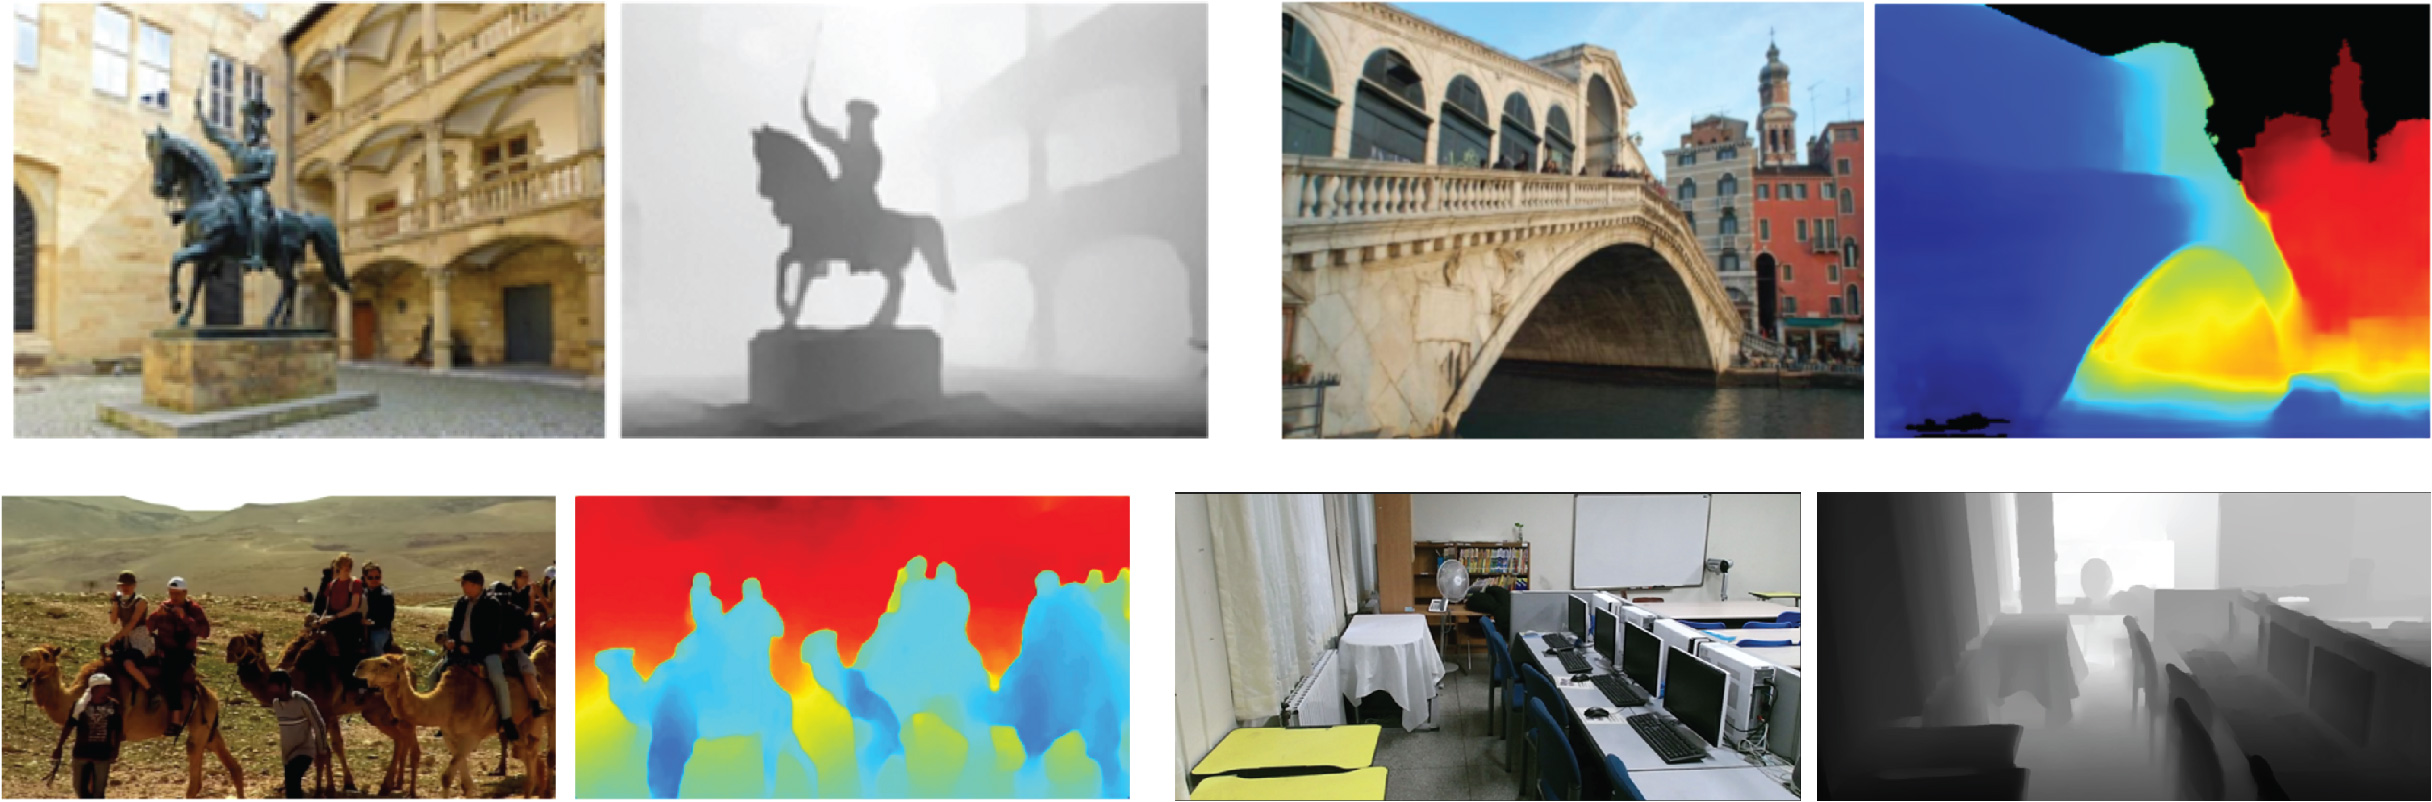
\includegraphics[width=1\linewidth]{figures/simplesystem_revisited/examples_training_midas.jpg}
    }
    \caption{Images and depth maps from the training set. {\em Source}: Image from \cite{Ranftl2022}.}
    \label{fig:examples_training_midas}
\end{figure}

As the model is trained with a diverse collections of data sources, there is an ambiguity on the overall scale, camera parameters, and stereo baselines. Therefore, the loss is defined in a way that it can be invariant to all those ambiguities. The invariant loss makes the training more robust, but it also makes the output less convenient to use.

To deal with the ambiguities mentioned before, the model is trained to predict disparity (inverse depth up to scale and shift). This means that we can not directly use the output. We need to convert it first into world coordinates.

\subsection{Adapting the Output}\label{sec:simple_system_revisited:adapting_the_output}


MiDaS returns disparity values, up to an unknown constant ($d_0$), but what we need are world coordinates ($X,Y,Z$) for each pixel. To perform this transformation, we will use what we learned in \chap{\ref{sec:camera_parameters}}. We will need to know the intrinsic and extrinsic camera parameters and also decide the value of $d_0$.

To translate the returned disparity for a given pixel $d\left[n,m \right]$ into depth values $z\left[n,m \right]$, we need to invert the disparity after adding the constant:

\begin{align}
    z \left[n,m \right] = \frac{1}{ d \left[n,m \right] + d_0}
\end{align}
Now we need to recover the world coordinates for every pixel.
Assuming a pinhole camera and using the depth $z \left[n,m \right]$ and the camera matrix $\mathbf{K}$, we obtain the 3D coordinates for a pixel with image coordinates $(n,m)$ in the camera reference frame as,
\begin{align}
    \begin{bmatrix}
        X \\
        Y \\
        Z
    \end{bmatrix}
    = z\left[n,m \right] \times \mathbf{K}^{-1} \times
    \begin{bmatrix}
        n \\
        m \\
        1
    \end{bmatrix}
    \label{eq:recoverworldcoord}
\end{align}


The camera parameters will have to account for the focal length, image size, camera center, and the camera rotation  with respect to the world coordinates:
\begin{equation}
    \mathbf{K} = \mathbf{M} \mathbf{R}
\end{equation}


The intrinsic camera parameters (using perspective projection) are:
\begin{align}
    \mathbf{M}
    =
    \begin{bmatrix}
        a & 0 & n_0 \\
        0 & a & m_0 \\
        0 & 0 & 1
    \end{bmatrix}.
\end{align}


The extrinsic camera parameters will model the 3D rotation, which is mainly around the $X$-axis (we will ignore the translation of the origin):
\begin{align}
    \mathbf{R}
    =
    \begin{bmatrix}
        1 & 0            & 0             \\
        0 & \cos(\theta) & -\sin(\theta) \\
        0 & \sin(\theta) & \cos(\theta)
    \end{bmatrix}.
\end{align}

%\marginnote{
\centerline{
    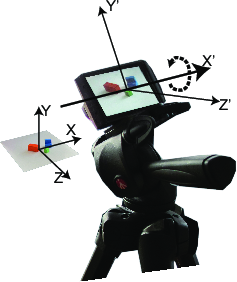
\includegraphics[width=.24\linewidth]{figures/simplesystem_revisited/projection-revisted.eps}
}
%}


%To be able to apply \eqn{\ref{eq:recoverworldcoord}} we need to define the parameters:
In order to apply \eqn{\ref{eq:recoverworldcoord}}, we need to define certain parameters:
$d_0$, $n_0$, $m_0$, $a$, and $\theta$.
Although we could determine these parameters using a calibration image, in this case, we'll opt for a simpler heuristic approach:
%We could recover these parameters using a calibration image. Instead, we will use a simpler heuristic here:
\begin{itemize}
    \item $d_0$: We will set this value to 0.
    \item $n_0,m_0$: Defines the camera center point, where $n_0=N/2$ and $m_0=M/2$, when $N \times M$ is the input image size.
    \item $a$: Accounts for the image size and the camera focal length. One standard setting is to make $a = N$, where $N$ is the image width.
    \item $\theta$: Represents the angle between the optical camera axis and the ground plane.
          %It would be possible to precisely estimate this angle by finding the direction of the surface normal in the pixels that correspond to the ground and measuring the angle with respect to the vertical axis. Here we will just set it to be $\theta = \pi / 4$ because that is close enough to the angle in which the pictures were taken.
          It would be possible to estimate this angle accurately by determining the direction of the surface normal in pixels corresponding to the ground and measuring the angle with respect to the vertical axis. However, for our purposes, we will simply set it to  $\theta = \pi / 4$, as this is approximately the angle at which the pictures were taken.

\end{itemize}

Now we are ready to use \eqn{\ref{eq:recoverworldcoord}} and the output of the system.

\section{From 2D Images to 3D}

%We will start with a simple image containing a single cube. 

Let's start running the model on the same input image that we used as a running example in \chap{\ref{chapter:simplesystem}}. We just need to apply the neural network to the input image, obtain the output disparity, and finally transform the disparity into world coordinates. We do not have to detect edges or any of the other features that we computed in \chap{\ref{chapter:simplesystem}}. Instead, the neural network has learned to compute whatever features it deems necessary to solve the task. We will not retrain the network using images from our simple visual world.


Just as we did in \chap{\ref{chapter:simplesystem}}, to show that the algorithm for 3D interpretation gives reasonable results, we can re-render the inferred 3D structure from different viewpoints.
\begin{figure}
    \centerline{
        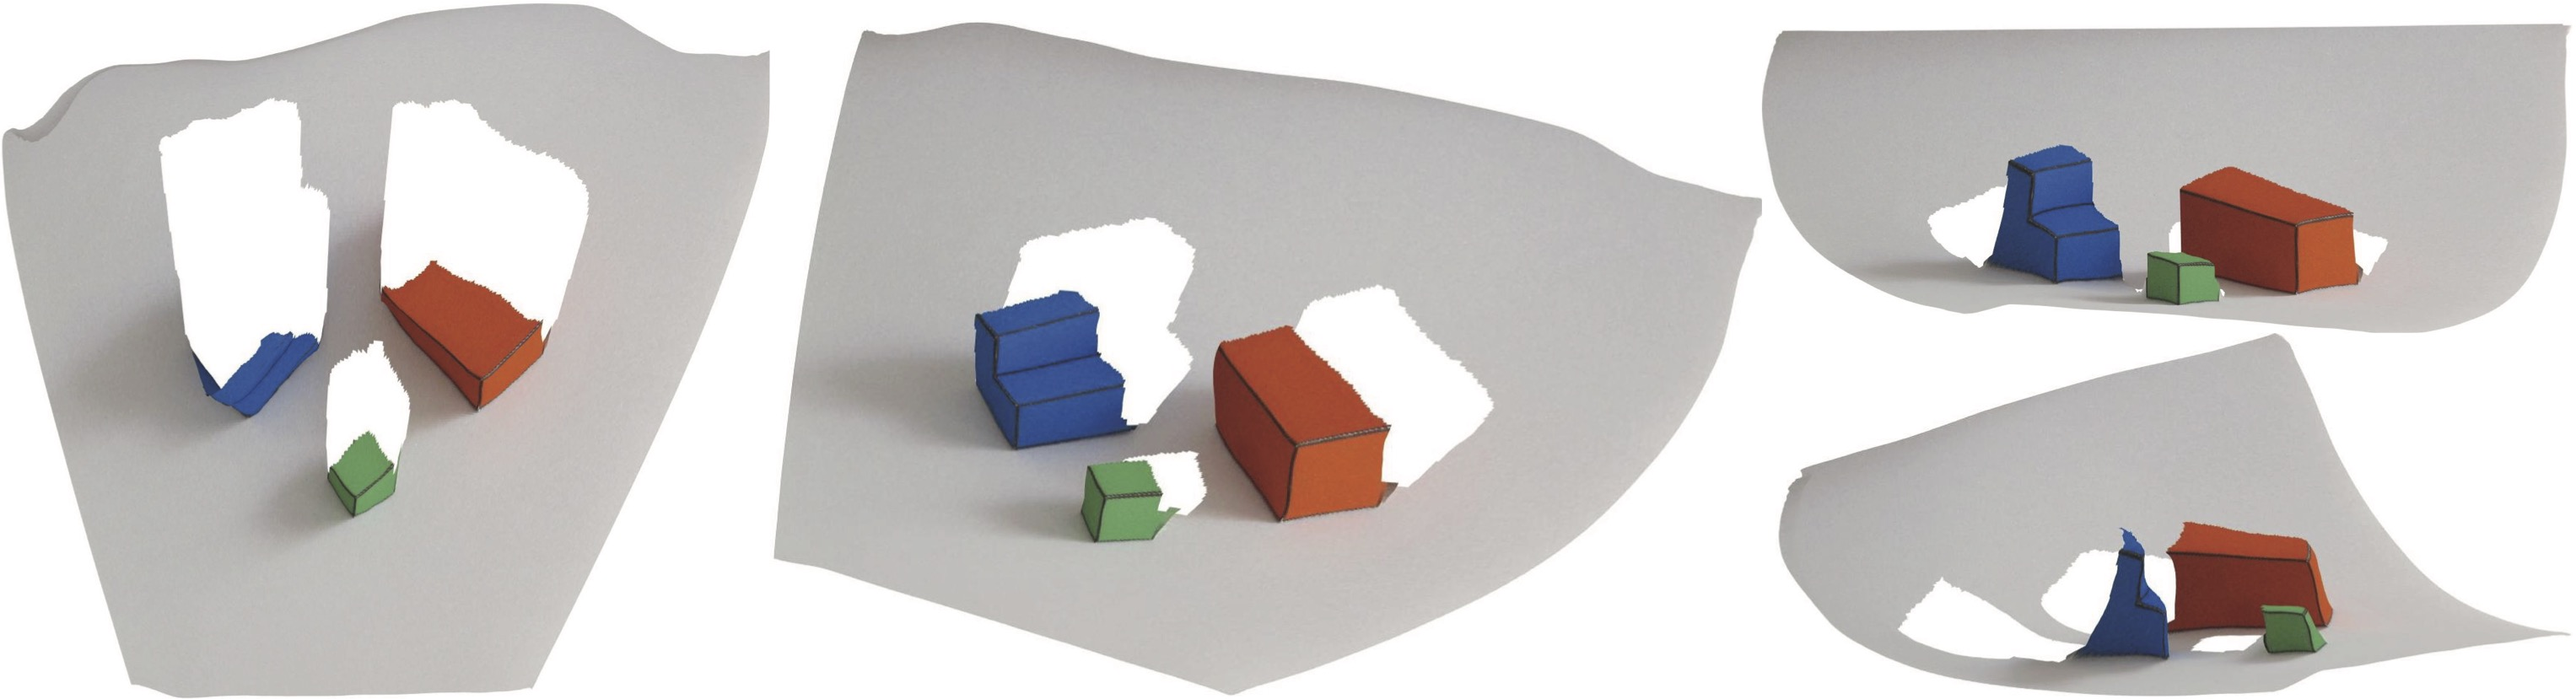
\includegraphics[width=1\linewidth]{figures/simplesystem_revisited/views_midas.jpg}
    }
    \caption{3D reconstruction using a pretrained model. The images show multiple view points of the reconstructed 3D scene from \fig{\ref{fig:simplesystem_revisited_img1}}.}
    \label{fig:views_midas}
\end{figure}

It is quite remarkable that it works somewhat well even though this system has been trained with natural images, which are quite dissimilar to the simple world we are using here. However, despite the surprising outputs, it is clear we cannot avoid a number of errors. For instance, the ground is not recovered as a flat surface; instead it seems to be concave. The cubes' edges are not straight and the faces are twisted instead of flat.

We can compare this result with the 3D images recovered using the algorithm we defined in \chap{\ref{chapter:simplesystem}}:
\begin{figure}
    \centerline{
        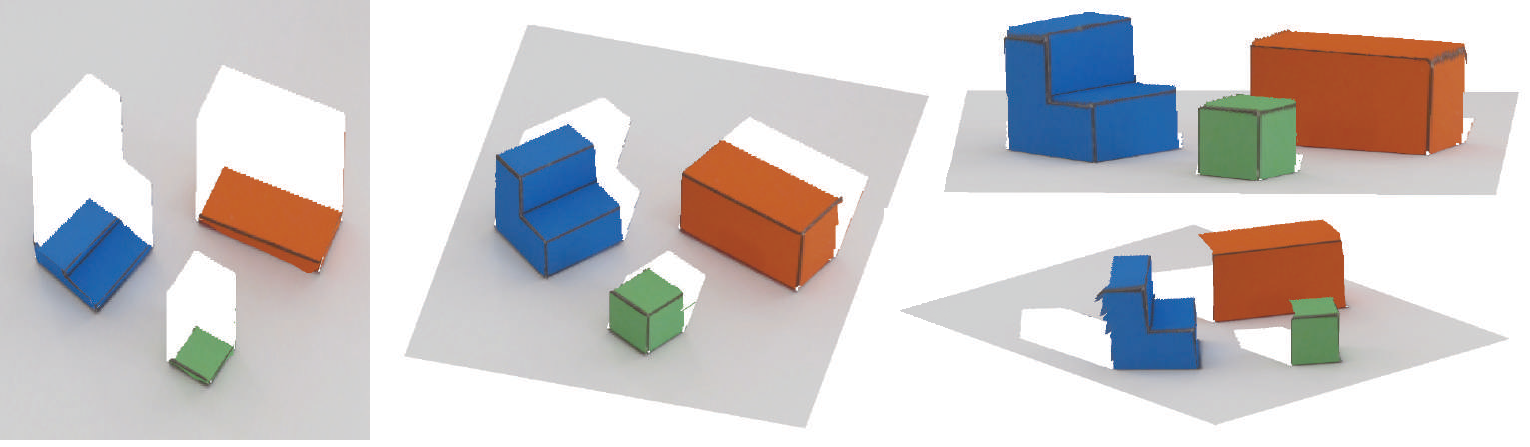
\includegraphics[width=1\linewidth]{figures/simplesystem/views.pdf}
    }
    \caption{3D reconstruction using the simple visual system from \chap{\ref{chapter:simplesystem}} for the same input image as in \fig{\ref{fig:views_midas}}.}
\end{figure}

However, while the learned-based model may have lost accuracy in this example that fits our simple world assumptions, it has gained in robustness and generalization.
%However, what the model has lost in accuracy in this example that fits our simple world assumptions, the trained model has gained in robustness and generalization. 
The following figure compares the results obtained running MiDaS (the learning-based approach) or the simple world model (a hand-crafted approach).
\begin{figure}
    \centerline{
        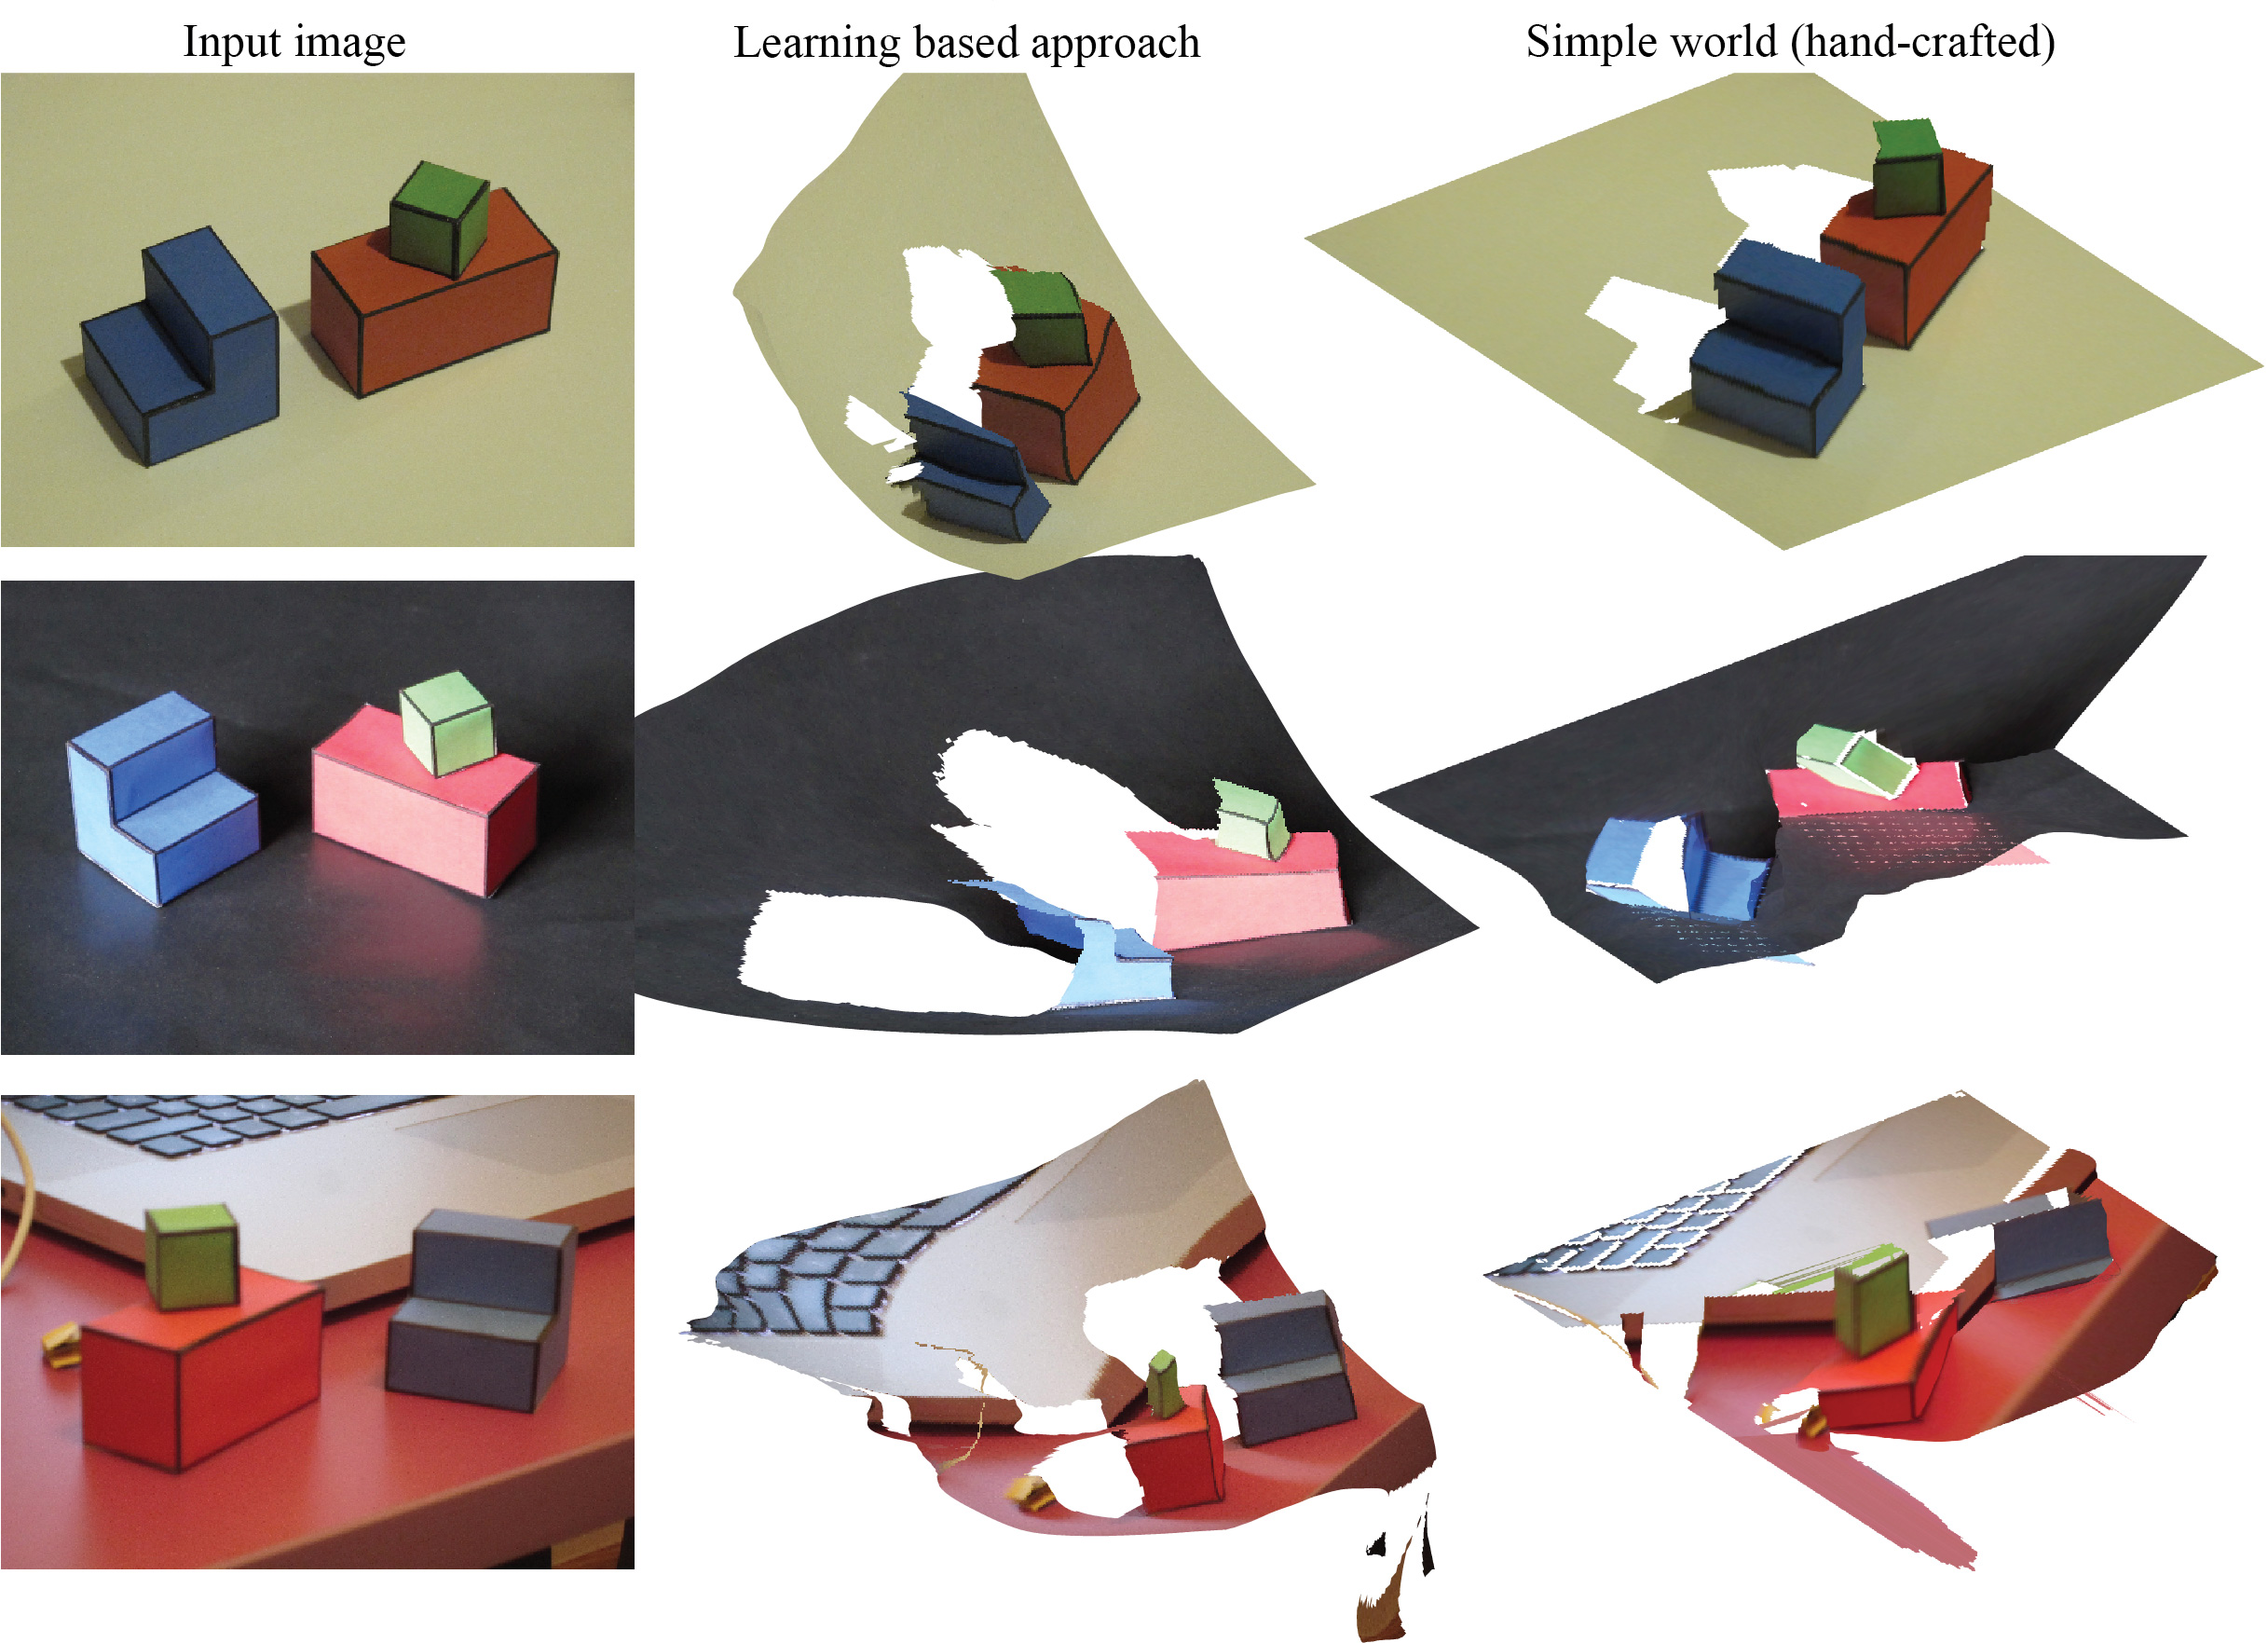
\includegraphics[width=1\linewidth]{figures/simplesystem_revisited/comparison_midas_simpleworld.jpg}
    }
    \caption{Out of domain generalization. For the pretrained model, these images might still be within the domain of the training, as it contained a very diverse set of natural images. The simple system model only works for the first example and breaks down for the rest, producing completely wrong reconstructions.}
\end{figure}
When the images fit the assumptions of the world model, the hand-crafted approach can produce beautiful results. However, it is very fragile, and poor illumination can break the output of the edge detectors, which results in a cascade of errors that propagate to the output. Conversely, the learning-based approach seems to produce results of good (although never perfect) quality regardless of the conditions. The hand-crafted approach completely fails even if we make a small change in the scene such as changing the ground plane from white to black.


\section{Large Language Model-based Scene Understanding}

Another option is to use GPT4-v \cite{openai2023gpt4v} to interpret the scene. GPT4-v can take as inputs images, and it allows asking questions about images. \Fig{\ref{fig:chatgpt_blockworld}} shows the result of asking GPT4-v to describe a simple world image.

This method is remarkably accurate, and now you know how it works. At one level Gpt4-v is a transformer trained on massive data, using an autoregressive modeling objective (\chap{\ref{chapter:transformers}}). On another level, you can understand what rules that transformer may have learned: it detects edges in its first few layers, uses filters that act like wavelets tiling Fourier space, and it reasons about perspective geometry to find vanishing points and estimate shape (as we have discussed along many chapters in this book).



\begin{figure}
    \centerline{
        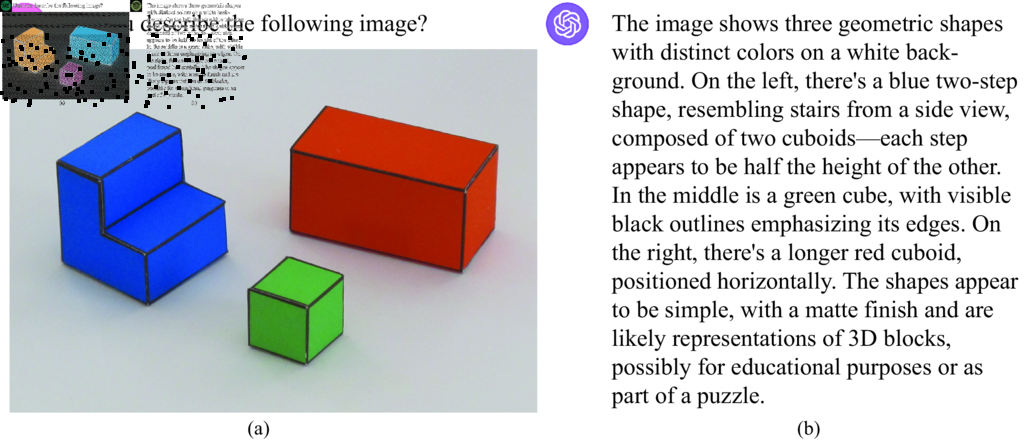
\includegraphics[width=1\linewidth]{figures/simplesystem_revisited/chatgpt_blockworld.eps}
    }
    \caption{(a) Input image and text prompt to ChatGPT. (b) Output by ChatGPT (Gpt4-v, version from Nov 21, 2023) when asked to describe the image from the simple world.}
    \label{fig:chatgpt_blockworld}
\end{figure}

But it's not all solved. Because if we reconstruct the image from this text, it looks not quite right: \fig{\ref{fig:chatgpt_blockworld2}}. What is missing? How would you improve it. As the field moves forward quickly, it is likely that this particular example will be fixed, but there will be other failures. And some of those failures will give clues to what is the next fundamental question that will need to be addressed.

\begin{figure}
    \centerline{
        \includegraphics[width=.5\linewidth]{figures/simplesystem_revisited/chatgpt_blockworld_2.eps}
    }
    \caption{Output by ChatGPT when asked to render a new image with the same elements as in \fig{\ref{fig:chatgpt_blockworld}}. This conversation is a continuation of the same chat from \fig{\ref{fig:chatgpt_blockworld}}.}
    \label{fig:chatgpt_blockworld2}
\end{figure}

\section{Unsolved Solved Computer Vision Problems}

Computer vision is making amazing progress, but beware of the {\bf unsolved solved computer vision problems}. For some vision task, it might appear as if there is one method that perfectly resolves the task. It might appear as if some foundational problems in computer vision are solved. It might often seem as if it is not possible to make progress regarding certain questions. But more often than not, it is just an illusion, and the solved problem was not really solved at all.

%And even when it was truly solved (and probably is not) remember that behind every solved problem there are many unsolved problems.
And even when a problem was genuinely solved (and probably is not), it's important to remember that for every solved problem, there are many unsolved problems lurking in the background.

\marginnote{When everything seems to be solved, remember that advances are the result of exploring new directions, with an open mind, and that creativity is a powerful tool.}

\section{Concluding Remarks}

What have we learned in this chapter? We learned that using a large pretrained model kind of works; it is not as clean as the results we had in \chap{\ref{chapter:simplesystem}}, but it works in situations where our simple heuristic method was breaking. And we can expect performances of future pretrained models to keep improving.

With the hand-crafted model presented in \chap{\ref{chapter:simplesystem}}, we had a comprehensive understanding of the mechanisms, assumptions, and limitations of our system. Another interesting advantage of the hand-crafted model is that it required no learning and no training data. Once the model was written down it was ready to work. It worked really well when the conditions were met, but it was fragile and unreliable as soon as we deviated from those conditions. Our hand-crafted model did not generalize outside the space defined by our assumptions. When the system failed, it was easy to point out exactly what went wrong with it, but knowing what was wrong was not helping in making it work better.

Conversely, the pretrained system for 3D reconstruction seems to have generalized to our setting, at least to some degree, and it is able to deal with configurations that were not part of our modeling assumptions. The pretrained model is robust to changes on illumination and does not rely on fragile operations such as edge detection or figure-ground segmentation. But somehow, equivalent operations might be taking place inside the network. Information about 3D is still mostly contained in the edges, and information has to be propagated from the edges and junctions to the flat surfaces. How does the pretrained model work exactly? Has it learned some of the heuristics we introduced by hand, or is it using other ones?

GPT4-v seems to be capable of recognizing the geometric figures and their spatial configuration but the integration with the rendering engine seems fragile and was not able to create a new image with the same elements (although it is very close!). But why did it fail?

The precise answers to these questions do not matter right now. The field is evolving quickly and many of those problems will be addressed over time. What matters is that you should challenge existing approaches, and find what the relevant questions are for whatever new systems you encounter.

With learning-based systems we find ourselves doing experiments similar to the ones performed by psychophysics in trying to understand the mechanisms implemented by the human visual system.

\begin{figure}
    \centerline{
        
\includegraphics[width=.06\linewidth]{figures/simplesystem_revisited/gibson_bird.eps}
    }
\end{figure}


\marginnote{
    \centerline{
        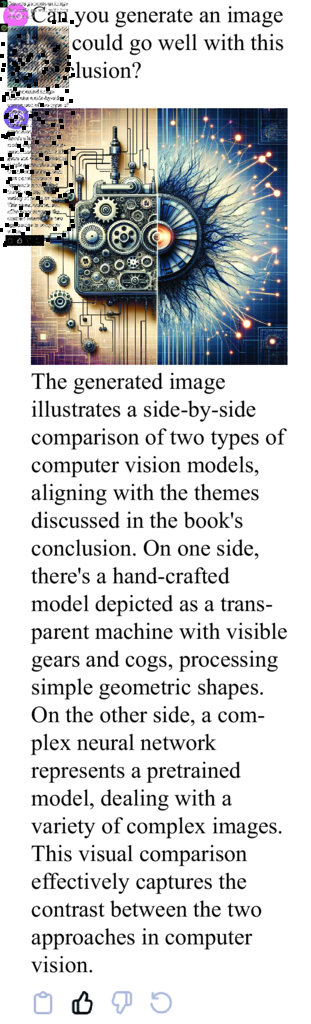
\includegraphics[width=.4\linewidth]{figures/simplesystem_revisited/conclusion_by_gpt4v.eps}
    }
}
